\chapter{Системный вызов open()}
Системный вызов \textit{open()} открывает файл, указанный в \textit{pathname}.
Если файл не существует и указан флаг \textit{O\_CREAT}, файл будет создан с правами доступа, указанными в \textit{mode}.

\begin{lstlisting}
#include <sys/types.h>
#include <sys/stat.h>
#include <fcntl.h>

int open (const char *pathname, int flags);
int open (const char *pathname, int flags, mode_t mode);
\end{lstlisting}

Системный вызов \textit{open()} возвращает дескриптор файла --- неотрицательное число, которое затем используется в системных вызовах \textit{read()} , \textit{write()} , \textit{lseek()} , и т.д. для ссылки на открытый файл.

Первый аргумент --- имя файла в файловой системе.
Второй аргумент --- режим открытия файла --- один или несколько флагов открытия, объединенных оператором побитового ИЛИ.
Могут быть использованны следующие флаги:
\begin{itemize}
	\item \textit{\textbf{O\_APPEND}} --- файл открывается в режиме добавления: перед каждой операцией записи файловый указатель будет устанавливать в конец файла;
	\item \textit{\textbf{O\_ASYNC}} --- включить ввод/вывод на основе сигналов (\textit{SIGIO} по умолчанию);
	\item \textit{\textbf{O\_CLOEXEC}} --- при вызове \textit{exec} файл не будет оставаться открытым;
	\item \textit{\textbf{O\_CREAT}} --- создать файл, если он не существует;
	\item \textit{\textbf{O\_DIRECT}} --- попытаться минимизировать эффект от кеширования ввода/вывода в/из этого файла;
	\item \textit{\textbf{O\_DIRECTORY}} --- вернуть ошибку, если файл не является каталогом;
	\item \textit{\textbf{O\_DSYNC}} --- операции записи будут выполняться в соответствии с требованиями для целостности данных;
	\item \textit{\textbf{O\_EXCL}} --- при использовании вместе с \textit{O\_CREAT} вызов \textit{open()} вернет ошибку, если файл уже существует;
	\item \textit{\textbf{O\_LARGEFILE}} --- позволяет открывать файлы, размер которых не может быть представлен типом \textit{off\_t};
	\item \textit{\textbf{O\_NOATIME}} --- не обновлять время последнего доступа к файлу;
	\item \textit{\textbf{O\_NOCITY}} --- если файл указывает на терминальное устройство, то оно не станет терминалом управления процесса, даже при его отсутствии;
	\item \textit{\textbf{O\_NOFOLLOW}} --- вернуть ошибку, если часть пути является символической ссылкой;
	\item \textit{\textbf{O\_NONBLOCK}} --- если возможно, открыть файл в неблокирующем режиме;
	\item \textit{\textbf{O\_PATH}} --- получить файловый дескриптор, который может быть использован для индикации расположения файла в файловой системе или для операций на уровне дескриптора;
	\item \textit{\textbf{O\_SYNC}} --- операции записи будут выполняться в соответствии с требованиями для целостности файла;
	\item \textit{\textbf{O\_TMPFILE}} --- создать неименованный временный файл;
	\item \textit{\textbf{O\_TRUNC}} --- если файл существует, его длина будет ''урезана'' до нуля;
\end{itemize}

Если вызов \textit{open()} создает новый файл, он будет создан с правами доступа, которые были переданы в \textit{mode}.
Для установки значения \textit{mode} определены следующие константы:
\begin{itemize}
	\item \textit{\textbf{S\_IRWXU}} --- права на чтение, запись, выполнение для пользователя;
	\item \textit{\textbf{S\_IRUSR}} --- права на чтение для пользователя;
	\item \textit{\textbf{S\_IWUSR}} --- права на запись для пользователя;
	\item \textit{\textbf{S\_IXUSR}} --- права на выполнение для пользователя;
	\item \textit{\textbf{S\_IRWXG}} --- права на чтение, запись, выполнение для группы;
	\item \textit{\textbf{S\_IRGRP}} --- права на чтение для группы;
	\item \textit{\textbf{S\_IWGRP}} --- права на запись для группы;
	\item \textit{\textbf{S\_IXGRP}} --- права на выполнение для группы;
	\item \textit{\textbf{S\_IRWXO}} --- права на чтение, запись, выполнение для остальных;
	\item \textit{\textbf{S\_IROTH}} --- права на чтение для остальных;
	\item \textit{\textbf{S\_IWOTH}} --- права на запись для остальных;
	\item \textit{\textbf{S\_IXOTH}} --- права на выполнение для остальных;
	\item \textit{\textbf{S\_ISUID}} --- бит \textit{set-user-ID};
	\item \textit{\textbf{S\_ISGID}} --- бит \textit{set-group-ID};
	\item \textit{\textbf{S\_ISVTX}} --- ''липкий'' бит;
\end{itemize}

\chapter{Используемые структуры}


\begin{lstlisting}[caption={Структура open\_flags}]
struct open_flags {
	int open_flag;
	umode_t mode;
	int acc_mode;
	int intent;
	int lookup_flags;
};
\end{lstlisting}

\begin{lstlisting}[caption={Структура filename}, showstringspaces=false]
struct filename {
	const char		*name;	/* pointer to actual string */
	const __user char	*uptr;	/* original userland pointer */
	int			refcnt;
	struct audit_names	*aname;
	const char		iname[];
};

struct audit_names {
	struct list_head	list;		/* audit_context->names_list */
	struct filename		*name;
	int			name_len;	/* number of chars to log */
	bool			hidden;		/* don't log this record */
	unsigned long		ino;
	dev_t			dev;
	umode_t			mode;
	kuid_t			uid;
	kgid_t			gid;
	dev_t			rdev;
	u32			osid;
	struct audit_cap_data	fcap;
	unsigned int		fcap_ver;
	unsigned char		type;		/* record type */
	bool			should_free;
};
\end{lstlisting}

\clearpage

\begin{lstlisting}[caption={Структура nameidata}]
struct nameidata {
	struct path	path;
	struct qstr	last;
	struct path	root;
	struct inode	*inode; /* path.dentry.d_inode */
	unsigned int	flags, state;
	unsigned	seq, next_seq, m_seq, r_seq;
	int		last_type;
	unsigned	depth;
	int		total_link_count;
	struct saved {
		struct path link;
		struct delayed_call done;
		const char *name;
		unsigned seq;
	} *stack, internal[EMBEDDED_LEVELS];
	struct filename	*name;
	struct nameidata *saved;
	unsigned	root_seq;
	int		dfd;
	kuid_t		dir_uid;
	umode_t		dir_mode;
} __randomize_layout;
\end{lstlisting}


\chapter{Схема выполнения системного вызова open()}

\begin{figure}[H]
	\center{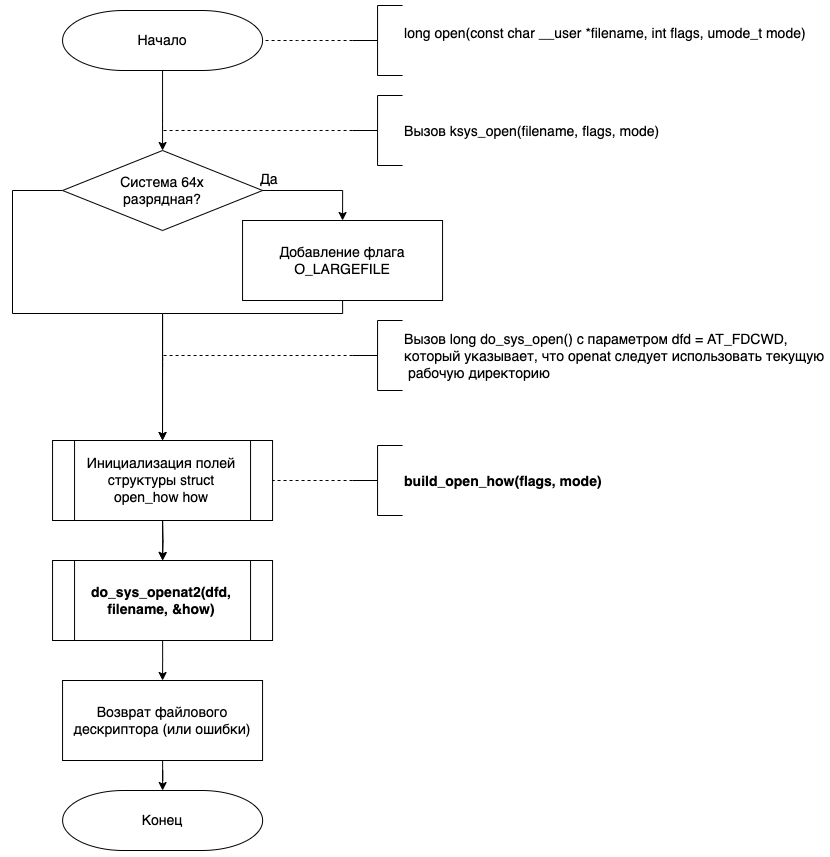
\includegraphics[width=1\textwidth]{img/open}}
	\caption{Схема алгоритма функции open()}
\end{figure}

\FloatBarrier

\begin{figure}[H]
	\center{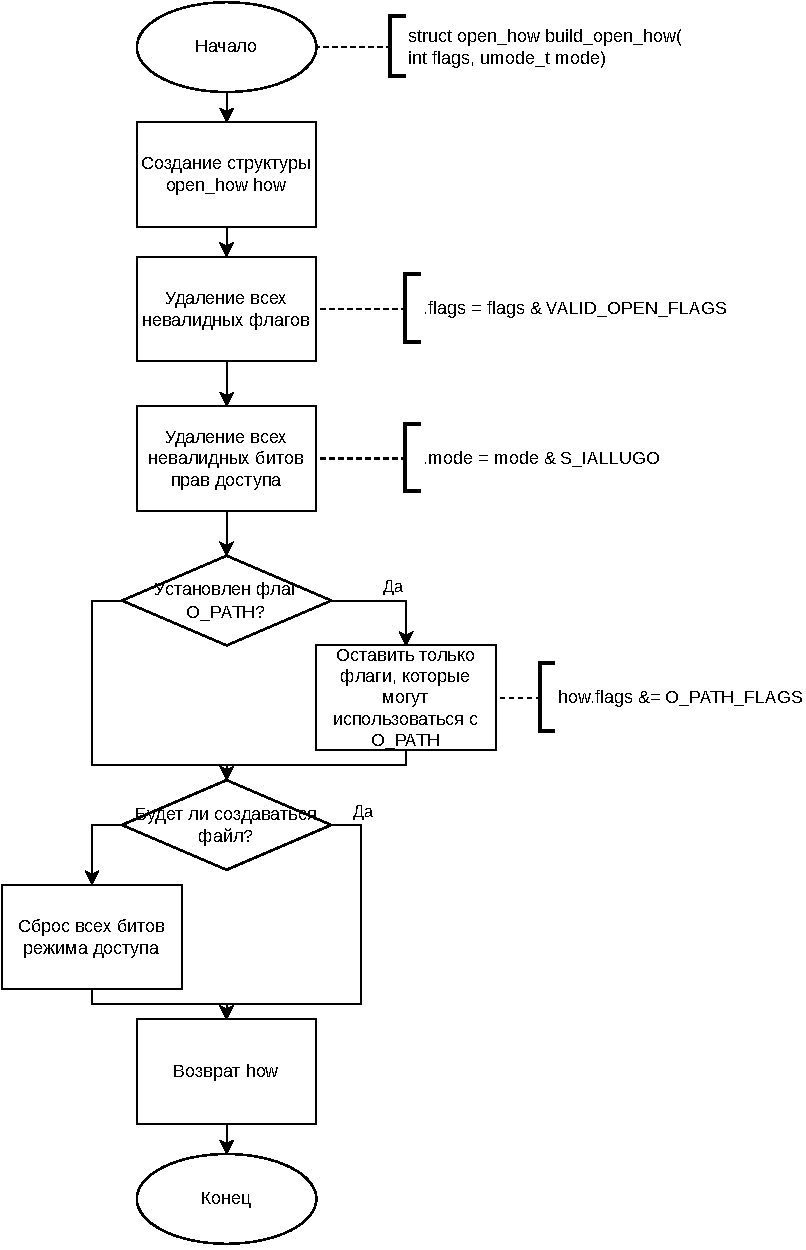
\includegraphics[width=0.9\textwidth]{img/build_open_how.pdf}}
	\caption{Схема алгоритма функции build\_open\_how()}
\end{figure}

\FloatBarrier

\begin{figure}[H]
	\center{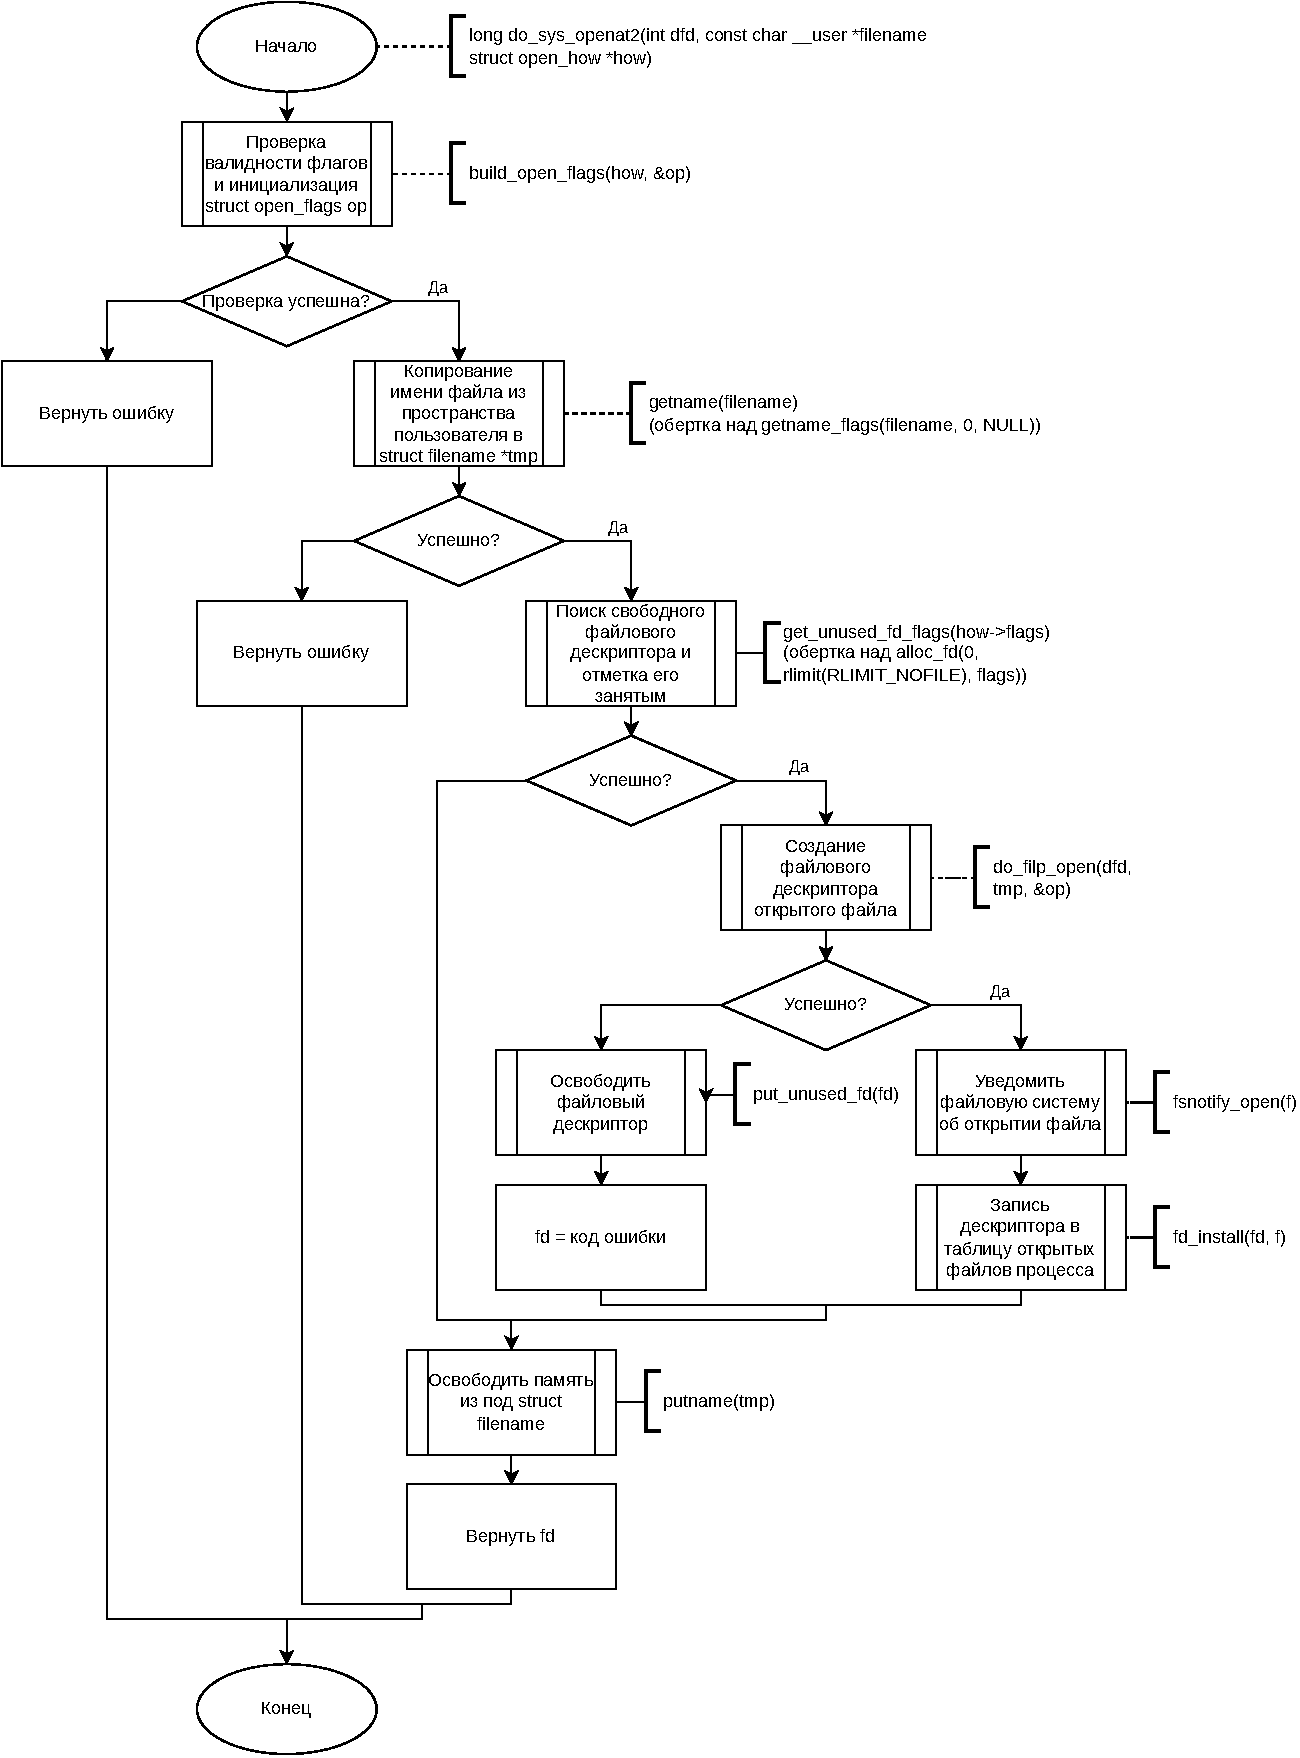
\includegraphics[width=1\textwidth]{img/do_sys_openat2.pdf}}
	\caption{Схема алгоритма функции do\_sys\_openat2()}
\end{figure}

\FloatBarrier

\begin{figure}[H]
	\center{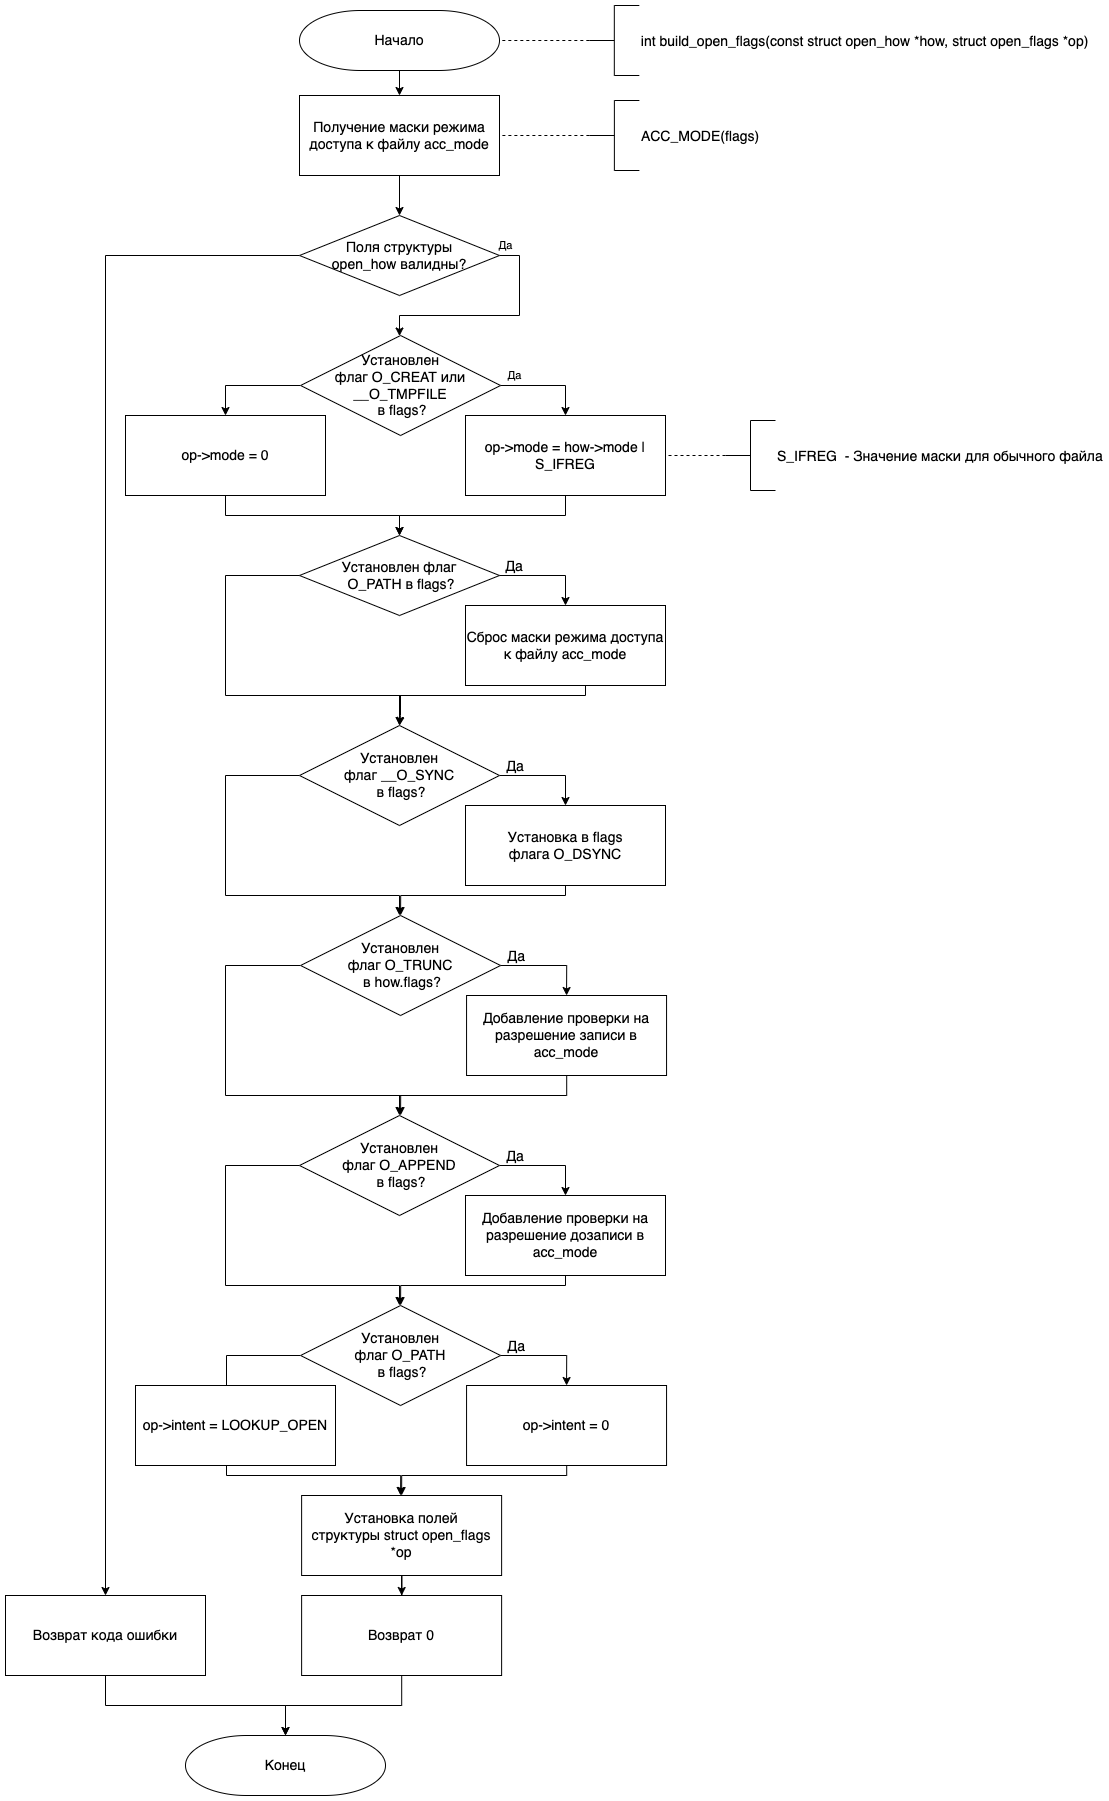
\includegraphics[width=0.9\textwidth]{img/build_open_flags.png}}
	\caption{Схема алгоритма функции build\_open\_flags()}
\end{figure}

\clearpage

\begin{figure}[H]
	\center{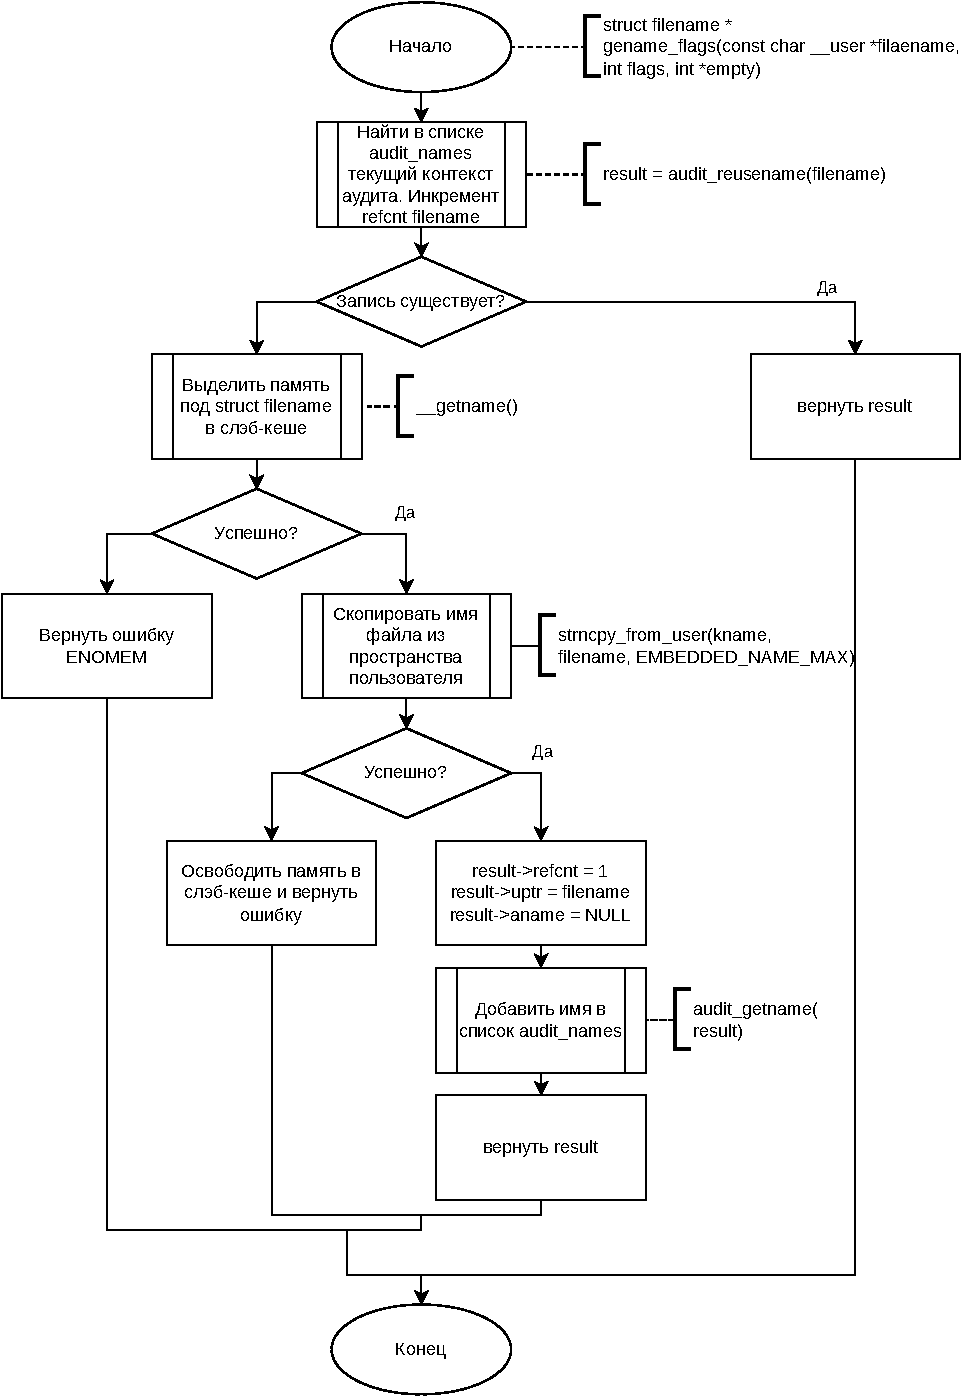
\includegraphics[width=1\textwidth]{img/getname_flags.pdf}}
	\caption{Схема алгоритма функции getname\_flags()}
\end{figure}

\begin{figure}[H]
	\center{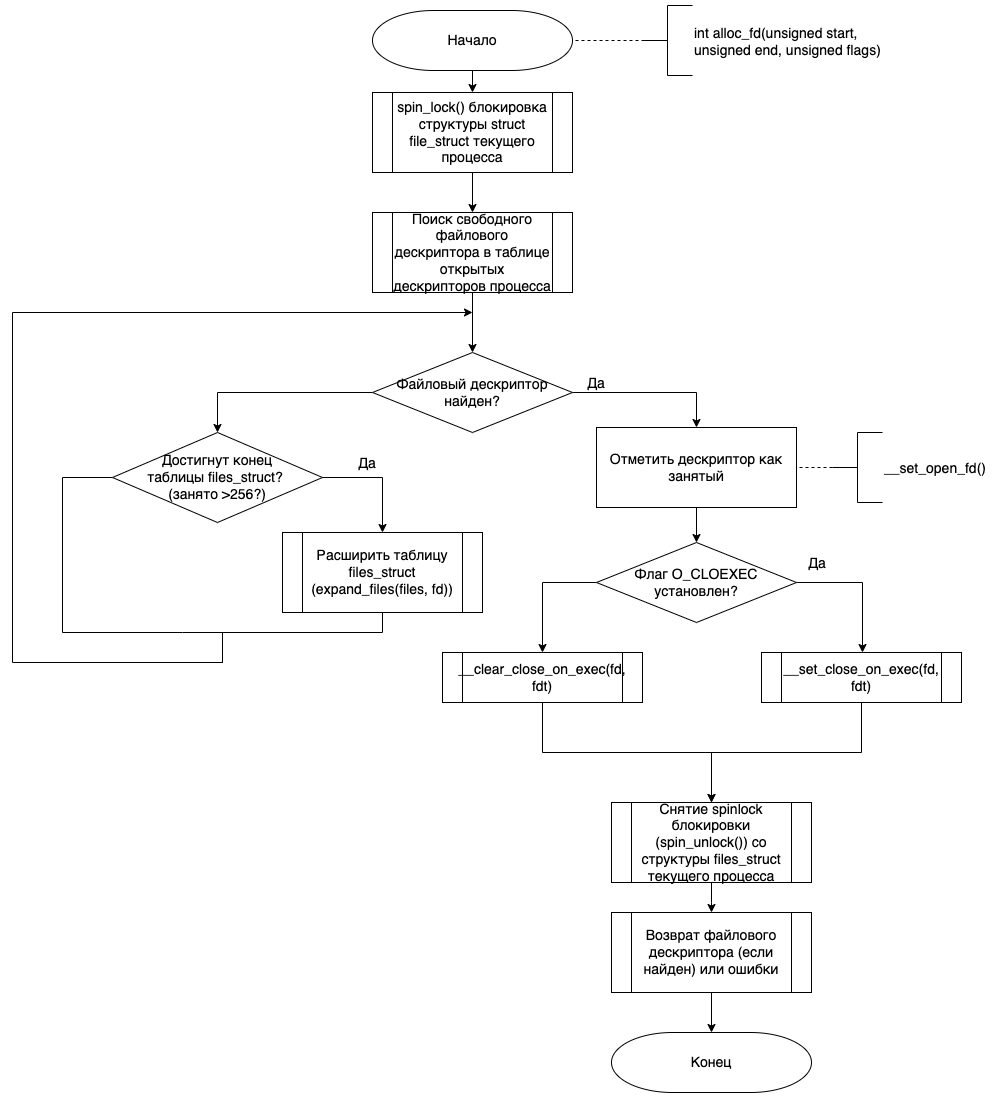
\includegraphics[width=1\textwidth]{img/alloc_fd.png}}
	\caption{Схема алгоритма функции \_\_alloc\_fd()}
\end{figure}

\begin{figure}[H]
	\center{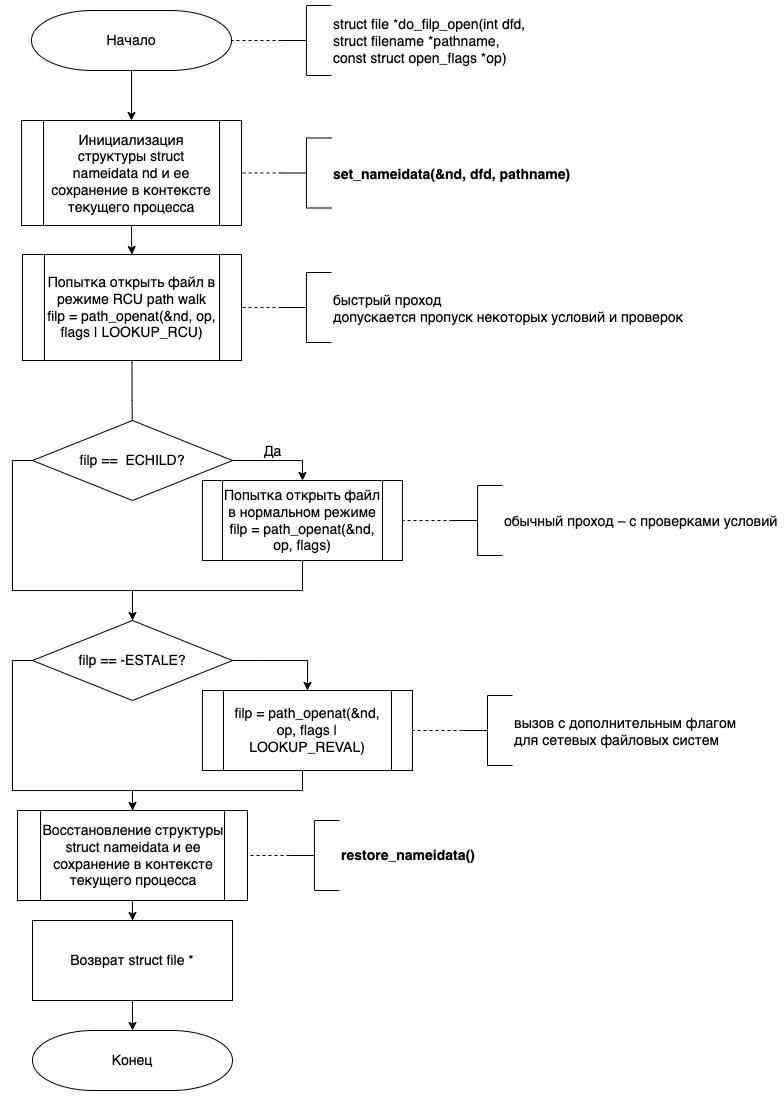
\includegraphics[width=0.85\textwidth]{img/do_filp_open.png}}
	\caption{Схема алгоритма функции do\_filp\_open()}
\end{figure}

\FloatBarrier

LOOKUP\_RCU --- флаг используется в системе VFS для указания , что операция
поиска должна выполняться с использованием RCU (Read-Copy-Update).

LOOKUP\_REVAL --- флаг для работы с NFS, указывает, что необходимо выполнить повторную проверку


\begin{figure}[H]
	\center{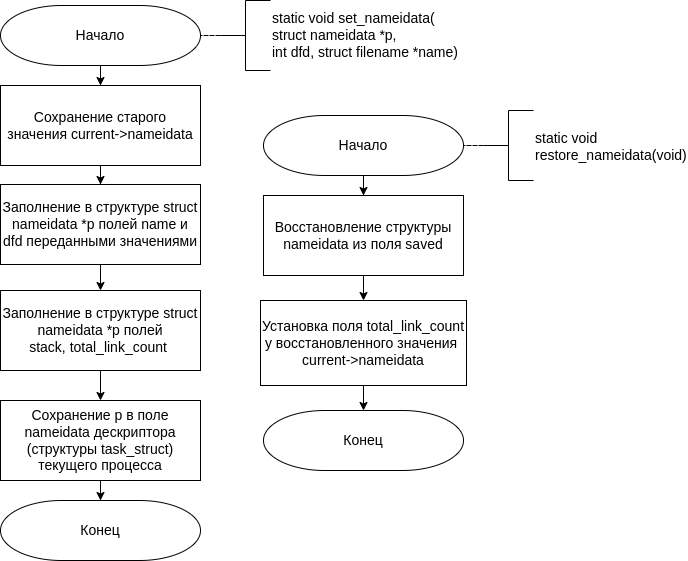
\includegraphics[width=1\textwidth]{img/nameidata.png}}
	\caption{Схемы алгоритмов функций set\_nameidata() и restore\_nameidata()}
\end{figure}

\begin{figure}[H]
	\center{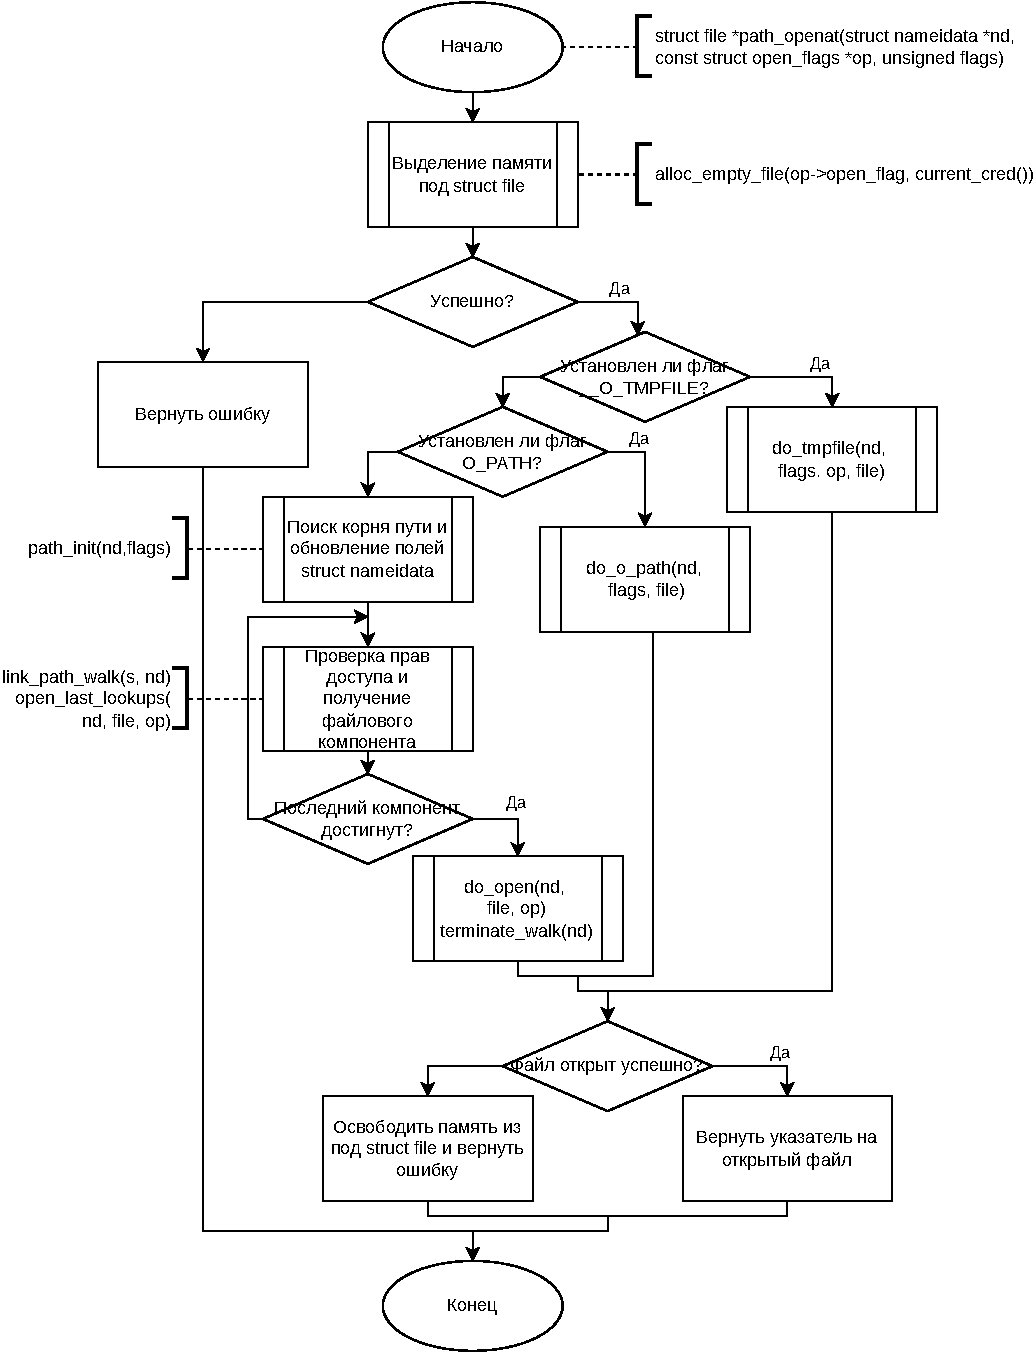
\includegraphics[width=1\textwidth]{img/path_openat.pdf}}
	\caption{Схема алгоритма функции path\_openat()}
\end{figure}

\begin{figure}[H]
	\center{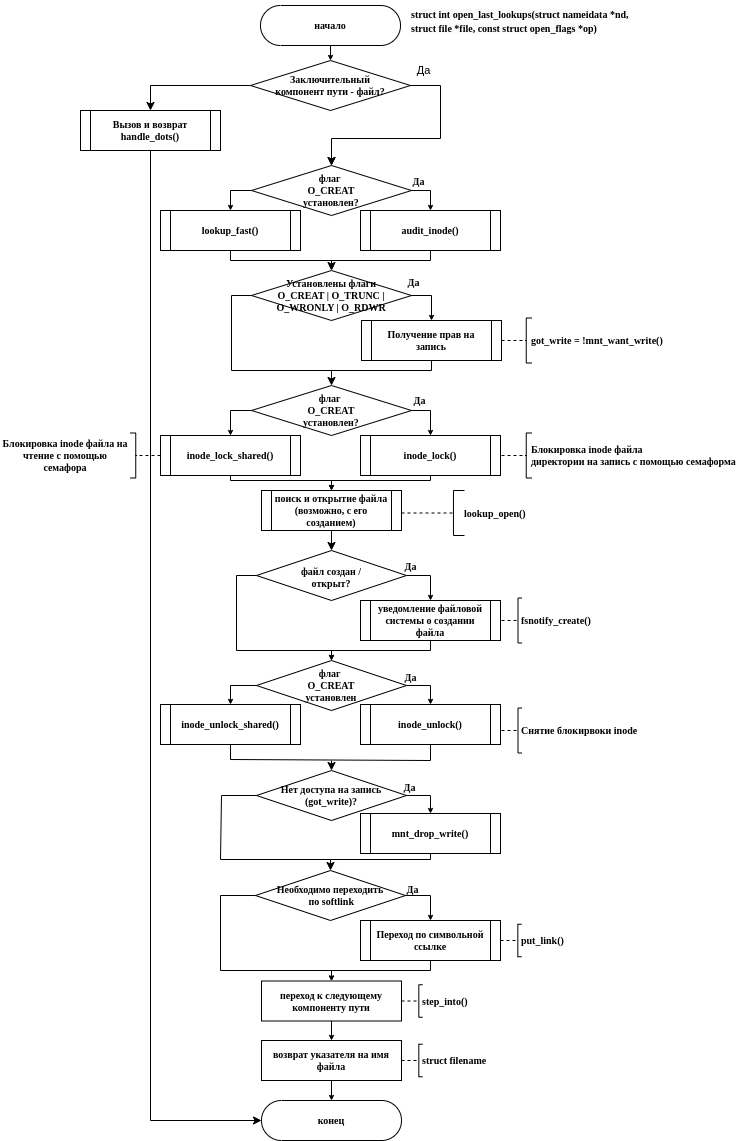
\includegraphics[width=0.9\textwidth]{img/open_last_lookups.png}}
	\caption{Схема алгоритма функции open\_last\_lookup()}
\end{figure}


\begin{figure}[H]
	\center{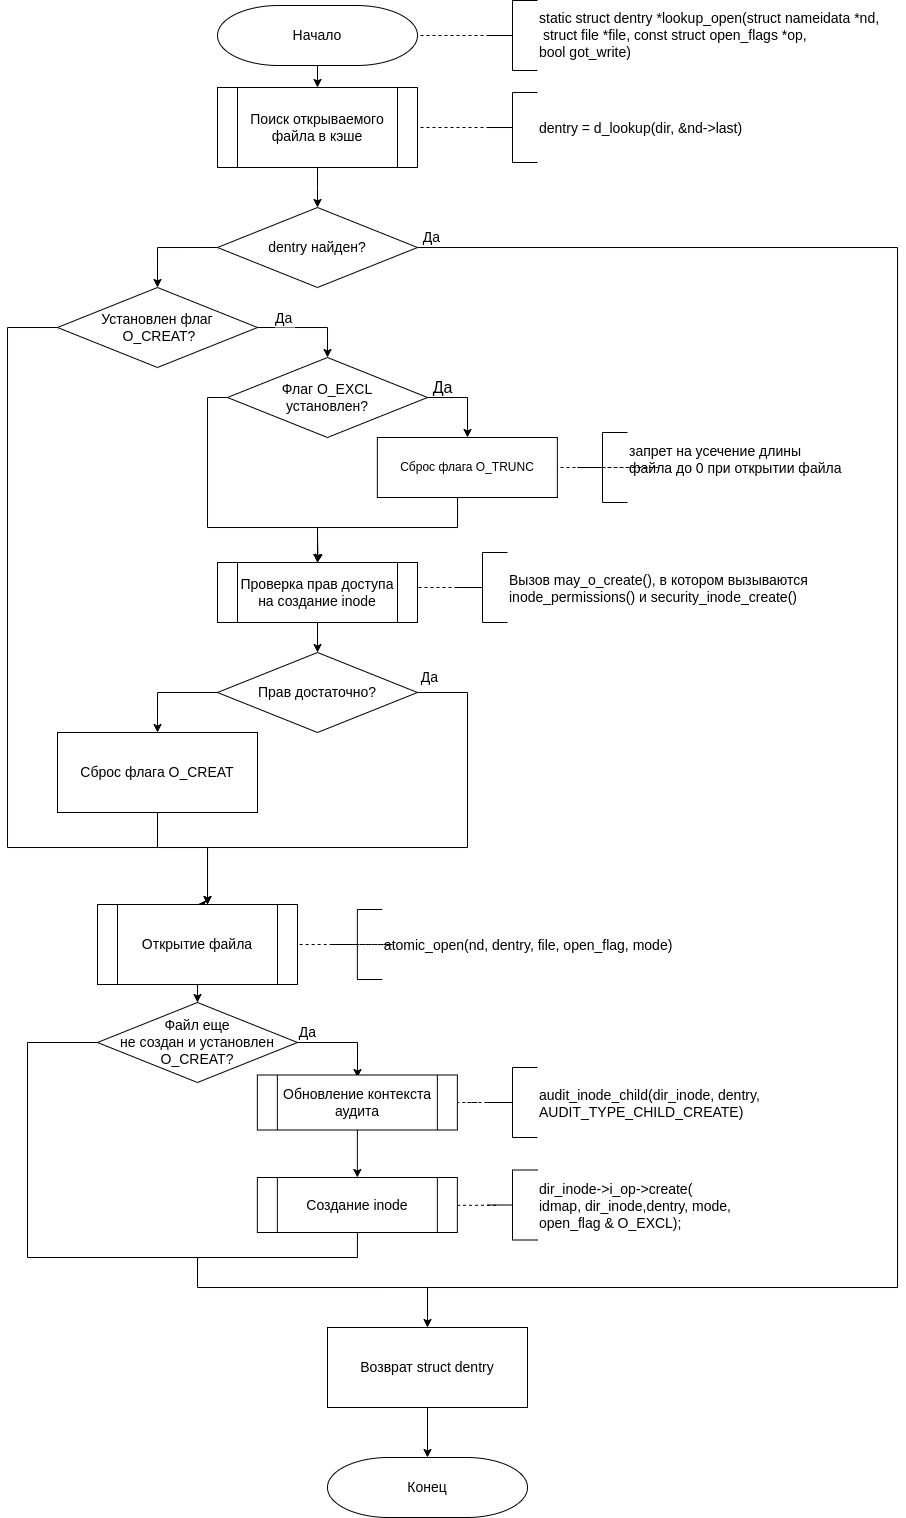
\includegraphics[width=0.82\textwidth]{img/lookup_open.png}}
	\caption{Схема алгоритма функции lookup\_open()}
\end{figure}

\begin{figure}[H]
	\center{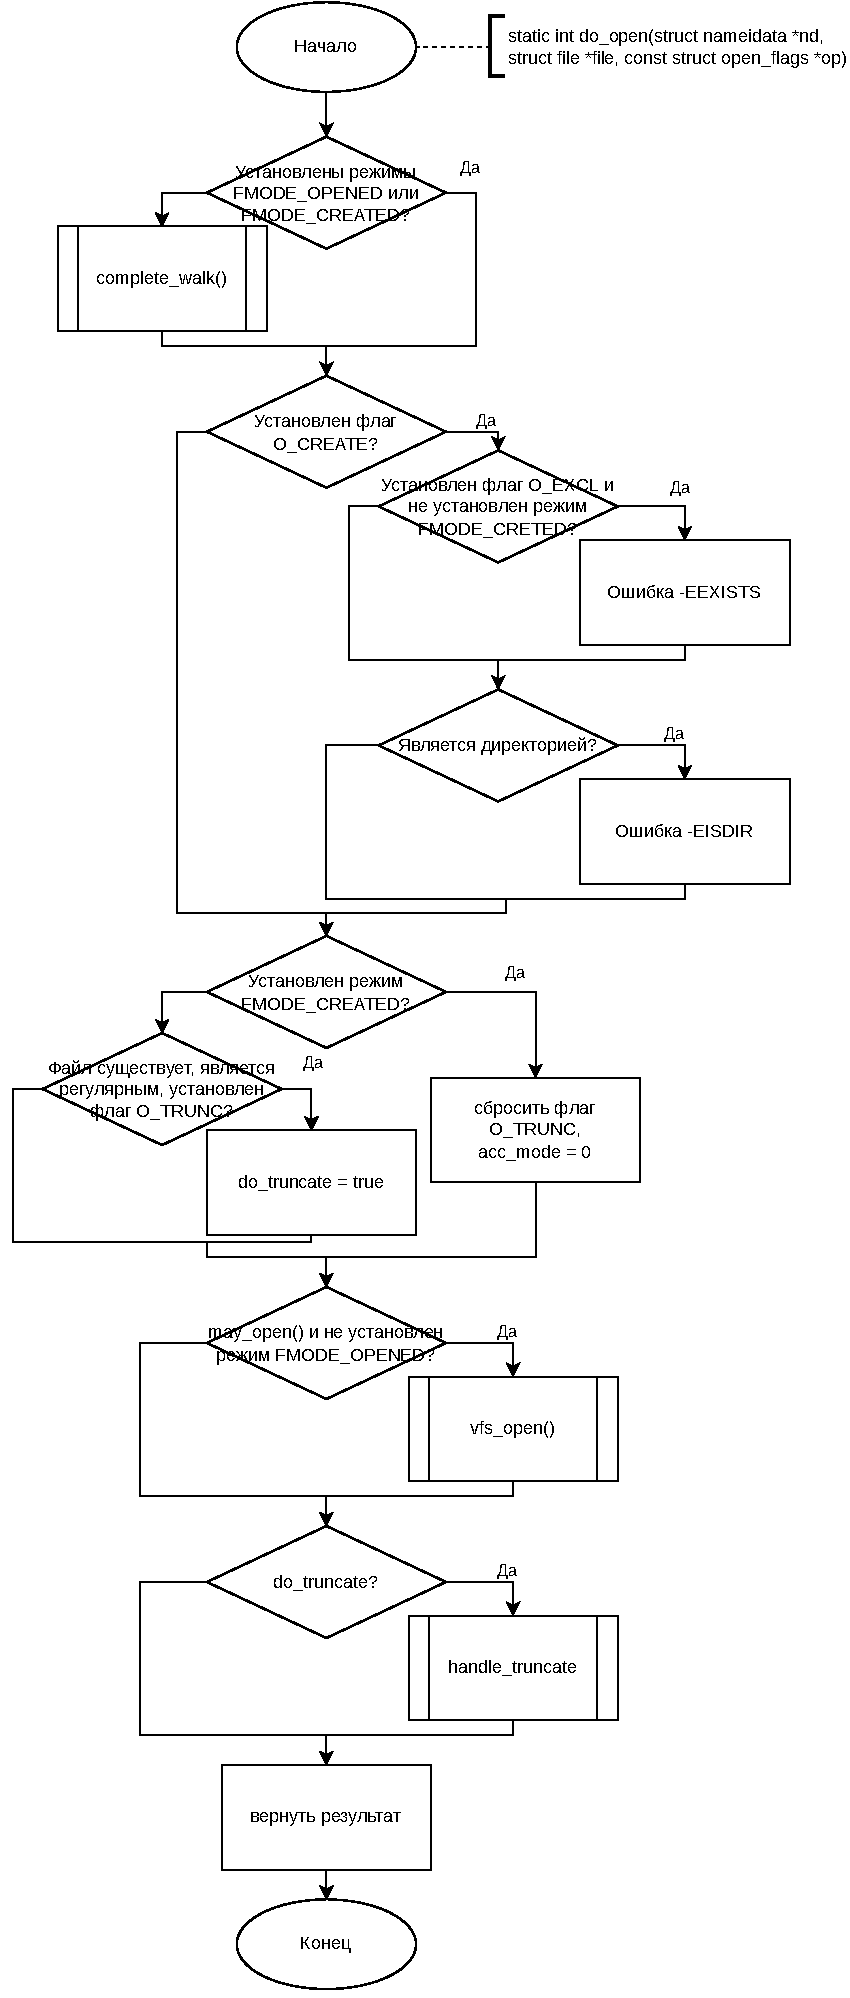
\includegraphics[width=0.61\textwidth]{img/do_open.pdf}}
	\caption{Схема алгоритма функции do\_open()}
\end{figure}
